\chapter{The Simulator}

\section{Introduction}

The project addresses the practical issues regarding the with the policy design of Dynamic Time-of-Use (dToU). This method incentivizes the users to increase or decrease their energy consumption with financial rewards through variable tariffs. It is also known as demand response (DR). The main reason to implement DR is to actively stabilize the system with user participation. On the other hand, users can maximize their energy cost savings by utilizing the incentives provided by the energy retailer.

For the research purpose, the Low Carbon London project was conducted in the United Kingdom (UK) from the beginning of 2011 to the end of 2014. The project was funded by energy consumers via Ofgem's Low Carbon Network Fund. The programme was UK's first dynamic-electricity-pricing trial for the residential sector. The trial was designed to study the impact of large scale dynamic load shifting on the system. In this trial, 5,567 households participated. Out of those, 1,122 households received the experimental dToU tariff that was in effect for the duration of 2013.

\section{Limitations of LCL dataset}
\label{limits-lcl}
The energy consumption data collected in the LCL project ranged for four years. The dToU experiments were only carried out for one year with around 20\% of the total participants. This imposes the limitations on the quality of information that the dataset can provide. The reasons are listed below:

\begin{enumerate}
    \item User adaption/learning curve
    \item Seasonality, Trends of time series
    \item The 'enthusiast effect' in the trial
\end{enumerate}

\subsection{User adaption curve (learning curve)}
\label{learning-curve}

The LCL project was first of its kind that was ran with UK residential energy consumers. The trials consisted of motivating people to change their energy consumption pattern, which essentially means that people had to change their life long habit of using their appliances in a certain manner. Therefore, it was natural to expect some resistance by the participating customers while adapting to the new major change in their lifestyle, introduced by the dynamic tariffs. As the original findings of LCL learning report say, "the performance is consistent with a slight reduction in demand response magnitude over the course of the trial". Additionally, to support this hypothesis, figure \ref{fig:learning-curve} shows the LCL data from January 2013 and November 2013. Remember that the dToU trials started in January 2013.


\begin{figure}[t!]
    \label{fig:learning-curve}
    \centering
    \begin{subfigure}{0.8\textwidth}
        \centering
        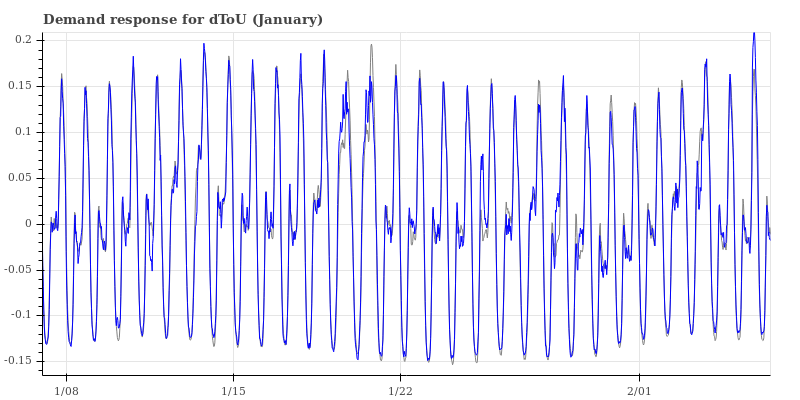
\includegraphics[height=2.2in]{img/DR-dToU-January.png}
        \caption{January: Aggregate single tariff user consumption(Grey line) and aggregate dToU tariff user consumption(Blue line)}
    \end{subfigure}%
     
    \begin{subfigure}{0.8\textwidth}
        \centering
        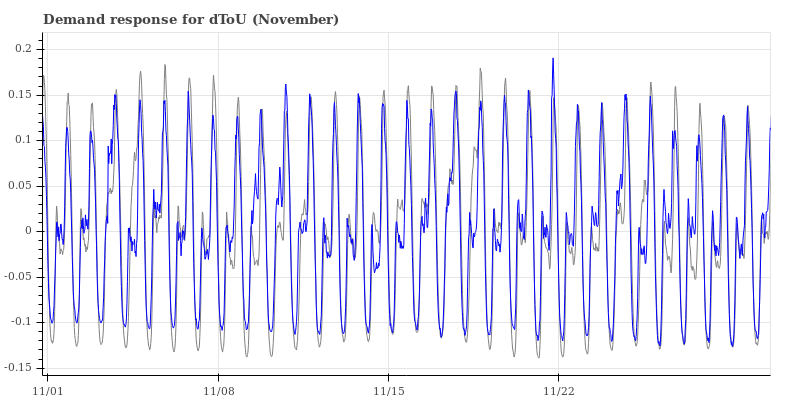
\includegraphics[height=2.2in]{img/DR-dToU-November.png}
        \caption{November: Aggregate single tariff user consumption(Grey line) and aggregate dToU tariff user consumption(Blue line)}
    \end{subfigure}
    \caption{Learning Curve for dToU tariff users}
\end{figure}


During the initial days of the trial, we can see a very small and irregular change in aggregate energy consumption. But over time, the participants of the trial started to positively change the energy usage pattern based on the dToU tariffs. The months of October and November experienced the greatest peak load shifting pattern during the trials. Of course, it would be irresponsible of the author to attribute the total load shift entirely to the above mentioned effect,  but the consistency in the load shift can be attributed to this effect. For example, weekly pattern in load shift is clearly visible and it can be argued that this shows the dToU tariff users have been consistent in their behaviour. This leads to the next issue about working with LCL data for time series prediction purpose, that is seasonality of time series data.

\subsection{Seasonality, Trends of time series}

Seasonality and trends are important characteristics of time series data. Seasonality can be defined as the linear or non-linear component that changes over time and repeats periodically. For energy usage time series data, the most visible seasonal factors are weekly seasonality and annual seasonal change (winter, spring etc.). The following plot shows the data of aggregate energy consumption of normal tariff users in LCL project collected from 2012 to 2014.

\begin{figure}[h]
    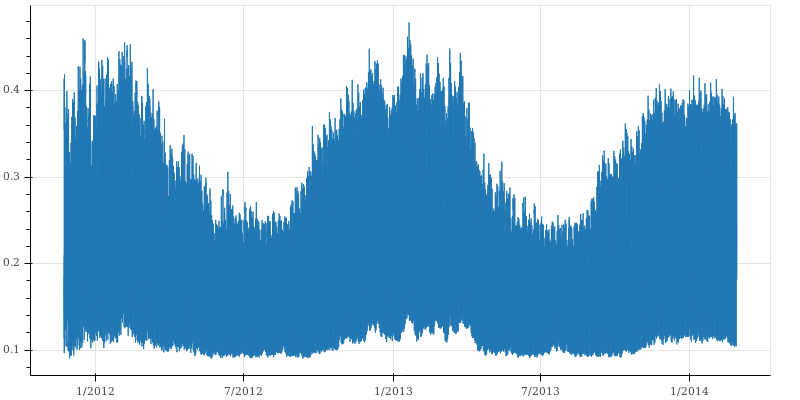
\includegraphics[width=0.8\textwidth]{img/timeseries-seasonality.png}
    \centering
    \caption{Seasonality of energy consumption pattern for residential users of LCL trials}
    \label{fig:aviko-design}
\end{figure}

The annual periodic changing pattern in energy consumption can be observed clearly. Usually, during summers the overall energy consumption drops due to the rise in ambient temperature. Whereas, during winters overall energy consumption increases due to falling in ambient temperature. These are the findings limited to the UK based on data and overall weather conditions. This user behaviour can be different for different regions/ countries based on local conditions. For this particular dataset, the dToU trials were conducted for the duration of one year. It will be a risky assumption to consider this data to be information-rich about user behaviour characteristics. In other words, even if the data captured the annual seasonality of energy usage pattern, there is no way to cross-validate that claim.

Similarly, the trial period is insufficient to understand any trends in the data. In time series, the trends are linear or non-linear components which do not repeat. In energy consumption data, trends can be listed as an overall increase in energy consumption over the years due to digitalisation, the rise of electric vehicles and increased electric heating systems. Another example of a non-linear trend is irregular load demand due to increasing rooftop solar installations.

\subsection{The 'novelty effect' in the trial}

This factor is mostly seen in the introduction of a new system or a new technology. The novelty effect seems contradictory to the human behaviour characteristic presented in section \ref{learning-curve} (learning curve), but it represents a different set of human traits which are motivated to act based on little or no experience with the system. The participants of the LCL trials were willingly participating in the project. The desire for active participation might have resulted in biased outcomes during initial weeks of trials. Therefore, using a machine learning model to learn user behaviour based on the dynamic tariff behaviour of users might not reflect actual response when implemented on a wide scale.

Based on the above concerns, it would be negligent on our side to base the experiment setup on the limited data of one year of user behaviour data. These aforementioned concerns call for the need for a simulator which can simulate historic conditions (based on available LCL dataset) and address the problem of the small LCL dataset by generating new data points. Also, the issue of calculating the load shifting can be solved by manually shaving the demand with some predetermined factor. Although this would not be an ideal solution to model user behaviour, it would be the first approach because of its simplicity.

% \section{Related work}


\section{Problem setting}
This section gives an overview of the proposed simulator (version-1). The simulator is based on the statistical knowledge gained by the LCL trials. This knowledge would be implemented for the generation of new data points by introducing the noise in the current dataset. Suppose $X$ denotes the aggregate user behaviour sequence for the normal tariff, $Y$ denotes the aggregate user behaviour sequence for a dToU tariff. $\phi$ is the set of parameters which represent the occupancy behaviour. $\alpha$ is the set of user action profile for a given tariff policy.

\begin{equation}
    X = f(\theta)
\end{equation}
    
\begin{equation}
     Y = h(X, \alpha)
\end{equation}

This architecture allows checking various conditions like alteration in the participating consumers, different climate conditions, various calendar effects (holidays, special events). The architecture is flexible and can be easily modified to study the future demand response by incorporating the increased penetration of home automation and electric vehicles.

\section{Effect of various parameters}
\subsection{User occupancy behaviour}
The LCL trials found that around 'x'(replace with actual \%) per cent of participating users had never reacted to dToU tariffs. From remaining user base, approximately \% of users reacted to each trial experiment. The above-mentioned two parameters are encoded in the simulator algorithm as two separate variables while selecting participating users

\subsection{Seasonal effect}
The energy usage pattern of residential users is heavily affected by seasonal weather. Hence, season is a major parameter which has impact on the energy consumption.

\subsection{Calendar effect}
Another parameter which affects the energy usage is day-of-week. High correlation is observed between the same day of weeks. 

\subsection{Tariff policy}
For this experiment design, a random tariff policy is generated within the constraints of peak hours mentioned in (LCL report). Currently, only high tariff signal is taken into account. The \texttt{48x1} vector of tariff values is generated, which is then used to calculate the user response.

During the LCL trials, it was found that some users engage earlier than the time of tariff change while others engage with some latency. When this process is considered as a stochastic process, one can expect a bell shaped curve for a graph of number of users engaged vs the timestamp of first high tariff signal. Such response is modelled in the simulator and demand response for every user is calculated individually.

\section{Data generator}
With the limitations explained in section \ref{limits-lcl}, there was need of designing a new way of generating more data points. This section talks about the methodology that is implemented in this project for generating new data points. Remember that the project only deals with the aggregate data of residential users, which means it is the average of the individual energy consumption by all the users.

For the context of this document, a data point is defined as 48 element array of values representing the half hourly aggregate energy usage of ToU tariff users for specific calendar (like day, month, season etc.) and weather (like temperature, dew point and pressure etc.) conditions.

\subsection{How to generate a 'new' data point?}
The one common way of generating new data point is adding white noise (Usually Gaussian) to the existing data points. But in the case of regression problem, white noise may erase some important characteristics of the timeseries, and will make the synthetic data point 'less realistic'. Therefore, the simulation might not simulate the real world conditions.

The other approach to introduce noise is to reduce the number of data points in the average. From the weak law of large numbers (also called Khinchin's law), the average of results obtained from large number of experiments (here, large number of users)  converges in probability towards the expected value (which can be considered as a average baseline consumption pattern). If machine learning model can converge quickly in probability towards the expected value, the complexity of the problem can be considered as low. Therefore, we are actively seeking to reduce the high correlation of data generated for similar conditions (in this case, weather and calendar conditions). From the above law, we can deduct that if the number of data points are reduced, then the average deviates from the expected value, thereby introducing noise in the final value.

The project uses the later methodology along with the incorporation of findings of the LCL project. LCL trials found out that only about 50\% of all the ToU tariff users deliberately run appliances other than water and space heating systems, at off-peak hours to save money. In other words, for our model, we can randomly select 50\% of ToU tariff users and introduce noise by above mentioned method. This detail of the study is useful for modelling the generator.